\documentclass{article}
\usepackage{authblk,graphicx}
\usepackage{xcolor,colortbl}
\usepackage{fancybox}% Enable the fancybox macro for landscape tables
\usepackage{multirow}

\definecolor{Gray}{gray}{0.85}
\definecolor{LightCyan}{rgb}{0.88,1,1}

\newcolumntype{b}{>{\columncolor{blue}}c}


\newcommand\Warning{%
 \makebox[1.4em][c]{%
 \makebox[0pt][c]{\raisebox{.1em}{\small!}}%
 \makebox[0pt][c]{\color{red}\Large$\bigtriangleup$}}}%

%% Caption command good for all figures, indecies, etc.
\newcommand{\mycaption}[3]{
\caption[#1]{\textsf{#2.} \label{#1} \small{\linespread{1}#3}}
}


\begin{document}
\title{ANITA-4 SIP Simulator Note}
\author{R.J. Nichol}
  
%\date{April, 2003}
\maketitle

%%\tableofcontents 

\section{Introduction}
The SIP Simulator is a CSBF laptop that performs the roll of the SIP for ground testing. The main SIP Simulator functions are:
\begin{itemize}
\item Receiving the high rate (TDRSS) data from the flight machine and redirecting it to the ground TDRSS machine
\item Receive the two low rate links (TDRSS and Iridium) from the flight machine and forward it to the ground TDRSS machine
\item Communicate with the Science Stack, reading housekeeping voltages and controlling the discrete relays.
\end{itemize}

\section{Hardware Interface}
The physical connections between the SIP Simulator laptop and the instrument box are a series of serial links, with MIL-38999 conenctors on the instrument box side and DB9 connectors on the SIP simulator side. The cables are described in Table~\ref{tab:sipSimCables}.

The serial (DB9) cables from the ANITA instrument box connector to a USB to Serial converter which is connected to the SIP Simulator. Most of the cables just directly connector to the short white CSBF serial cables. The one exception is the Science Stack cable which is connected via a serial isolator. Table~\ref{tab:usbSerial} lists the various connections and the Windows Comm. Port.

\begin{table}[hbt]
  \centering
  \begin{tabular}{| c | c | b | c | c | l|}
    \hline
    \rowcolor{LightCyan}
Filter Pin Conn. & Pin &  &Serial Conn. & Pin & Comment \\
\hline
B98­S Science Stack & A & & DB9-M Sci. Stack & 4 &  Shield \\
B98­S Science Stack & B & & DB9-M Sci. Stack & 6 & RX IN \\
B98­S Science Stack & C & & DB9-M Sci. Stack & 7 & RX RTN \\
B98­S Science Stack & D & & DB9-M Sci. Stack & 8 & TX OUT \\
B98­S Science Stack & E & & DB9-M Sci. Stack & 9 & TX RTN \\
\hline
    \rowcolor{LightCyan}
Filter Pin Conn. & Pin &  & Serial Conn. & Pin & Comment \\
\hline
B4­S High Rate & A & & DB9-F High Rate 1 & 2 & TX \\
B4­S High Rate & B & & DB9-F High Rate 2 & 2 & TX \\
B4­S High Rate & C & & DB9-F High Rate 1 & 5 & GND \\
B4­S High Rate & D & & DB9-F High Rate 2 & 5 & GND \\
\hline
    \rowcolor{LightCyan}
Filter Pin Conn. & Pin &  & Serial Conn. & Pin & Comment \\
\hline
B98­S Low Rate & A & & DB9-F Low Rate 1 & 3 & RX \\
B98­S Low Rate & B & & DB9-F Low Rate 1 & 2 & TX \\
B98­S Low Rate & C & & DB9-F Low Rate 1 & 5 & GND \\
B98­S Low Rate & D & & DB9-F Low Rate 2 & 3 & RX \\
B98­S Low Rate & E & & DB9-F Low Rate 2 & 2 & TX \\
B98­S Low Rate & F & & DB9-F Low Rate 2 & 5 & GND \\
\hline
  \end{tabular}
  \caption{The SIP Simulator cables, note the RX and TX are from the flight computer's point of view. High Rate 2 is not currently used but could in principle provide a redundant link to the SIP or SIP simulator.}
  \label{tab:sipSimCables}
\end{table}

\begin{table}[hbt]
  \centering
  \begin{tabular}{| c | c | c | c |}
    \hline
    \rowcolor{LightCyan}
ANITA Serial & Intermediary & USB-to-Serial & COMM \\
\hline
GND Data & n/a  & 1 & 21 \\
GND CMD & n/a & 2 & 22 \\
Low Rate 1 & n/a  & 3 & 23 \\
Low Rate 2 & n/a & 4 & 24 \\
High Rate 1 & n/a & 5 & 25 \\
Science Stack & Serial Isolator & 6 & 26 \\ 
\hline
  \end{tabular}
  \caption{The SIP Simulator serial connections on the USB-to-Serial converter. }
  \label{tab:usbSerial}
\end{table}

\section{SIP Simulator Configuration}
There are a number of SIP simulator configuration files that have been set up for ANITA. These configuation files are listed in the Appendix of this document. It is particularly important that the Science Stack addresses are correctly set (CMD F7 and Housekeeping F3), if these are not set correctly the Science stack communication will fail as though the serial cable is not connected.

\clearpage
\section{Using the SIP Simulator}
\subsection{Starting the SIP Simulator}
The SIP Simulator Lab View programs need to be started once the SIP Simulator Windows laptop has booted. Figure~\ref{fig:screenShot} shows the Windows desktop and the SIP Simulator icon.
  \begin{figure}[hbt]
    \centering
    \resizebox{\textwidth}{!}{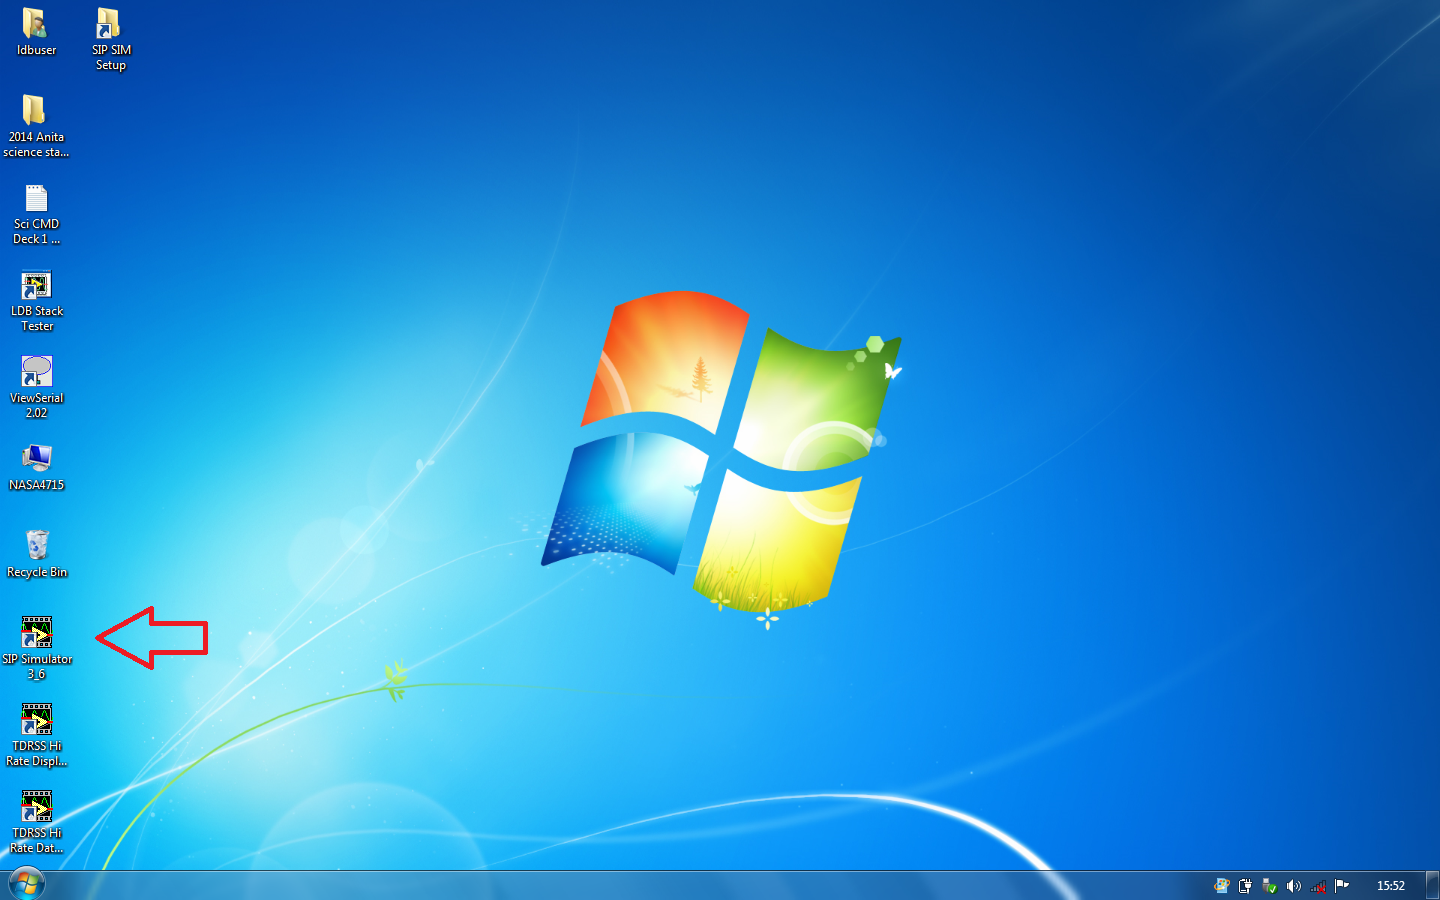
\includegraphics{screenShot.png}}
    \caption{The SIP Simulator Desktop screen. To start the SIP Simulator LabView program double-click on the icon illustrated by the red arrow.}
    \label{fig:screenShot}    
  \end{figure}

  Figure~\ref{fig:MainWindow} shows the Main Window of the SIP Simulator Lab view program. The Controls panel in the top left shows a list of auxilliary windows that can be opened by double-clicking. The Diagnostics window in the top right shows a log of the progress. The {\verb No reply from science housekeeping deck} indicates a problem, in this case the instrument and science stack were disconnected from the power supply and battery.
  
  \begin{figure}[hbt]
    \centering
    \resizebox{\textwidth}{!}{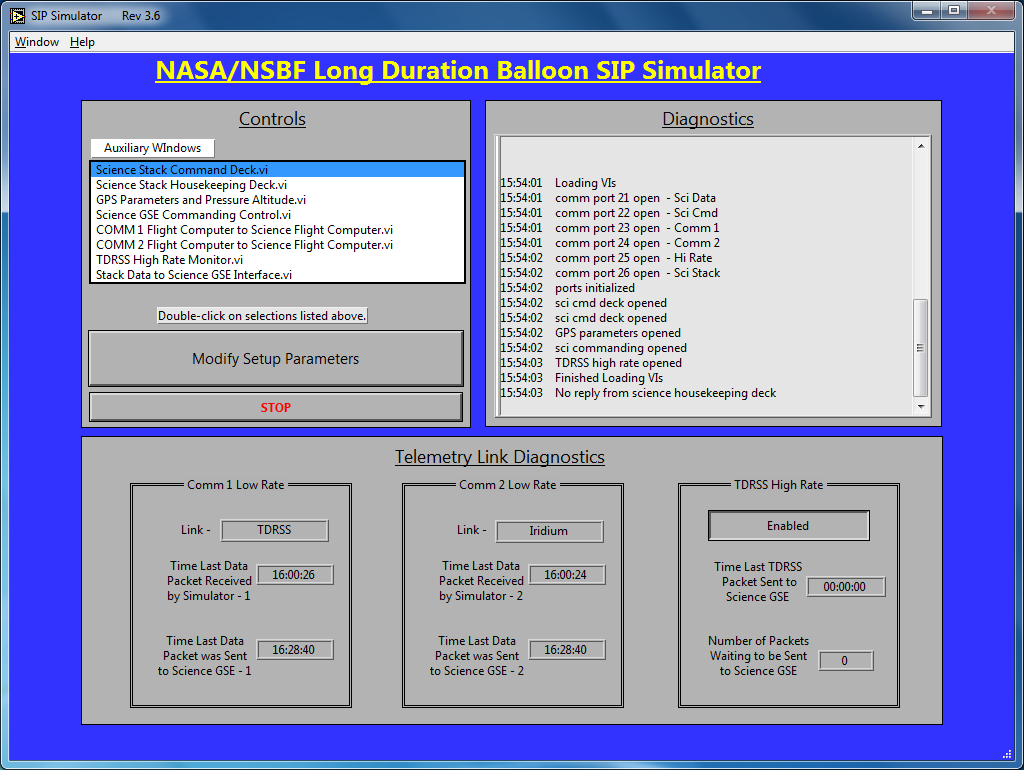
\includegraphics{MainWindow.png}}
    \caption{The main SIP Simulator window.}
    \label{fig:MainWindow}    
  \end{figure}

  \clearpage
  \subsection{Turning the instrument on or off with the SIP Simulator}

{\large \Warning \textit{ Do not send \textbf{AMPA EN ON} unless you absolutely know what you are doing and have received approval from a higher power to ensure this will not damage the instrument.} \Warning }
  
  
  To turn the instrument on using the science stack relays, we use the {\verb Science Stack Command Deck.vi}. Double-clicking brings up the Science Discrete Command Window, as shown in Figure~\ref{fig:CommandWindow}.
  \begin{figure}[hbt]
    \centering
    \resizebox{\textwidth}{!}{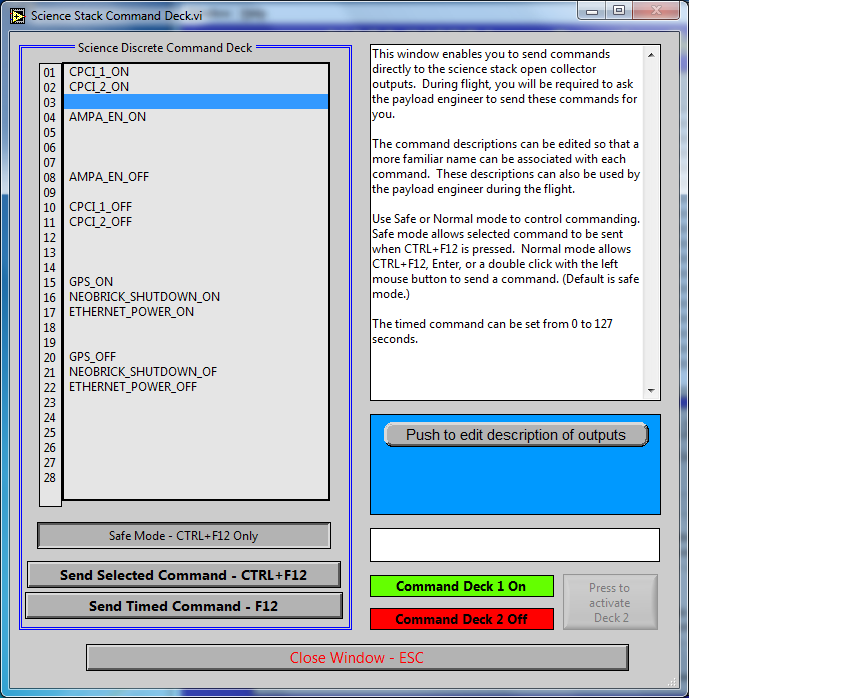
\includegraphics{commandWindow.png}}
    \caption{The SIP Simulator Science Stack Command Window.}
    \label{fig:CommandWindow}    
  \end{figure}

  To send a command:
  \begin{enumerate}
  \item Click on the command name, e.g. GPS ON, to highlight it in blue.
  \item Click on the {\verb Send Selected Command} button.
  \end{enumerate}
  if you get a message saying no reply from science command deck then something has gone wrong.
\newpage
  The approved ANITA-4 turn on sequence is:
  \begin{enumerate}
  \item \textbf{GPS ON}
  \item \textbf{ETHERNET ON}
  \item \textbf{CPCI1 ON}    
  \end{enumerate}

  The approved ANITA-4 turn off sequence is:
  \begin{enumerate}
  \item \textbf{GPS OFF}
  \item \textbf{ETHERNET OFF}
  \item \textbf{CPCI2 OFF}
  \item \textbf{CPCI1 OFF}    
  \end{enumerate}
    
  \subsection{Monitoring the instrument using the SIP Simulator}
  The SIP Simulator provides limited monitoring of the instrument. Figure~\ref{fig:hkWindow} shows the Housekeeping window which can be used to monitor the PV (Power Supply) and +24V (Battery) voltages and currents. These are only available when the insrument is switched on.
  
  \begin{figure}[hbt]
    \centering
    \resizebox{\textwidth}{!}{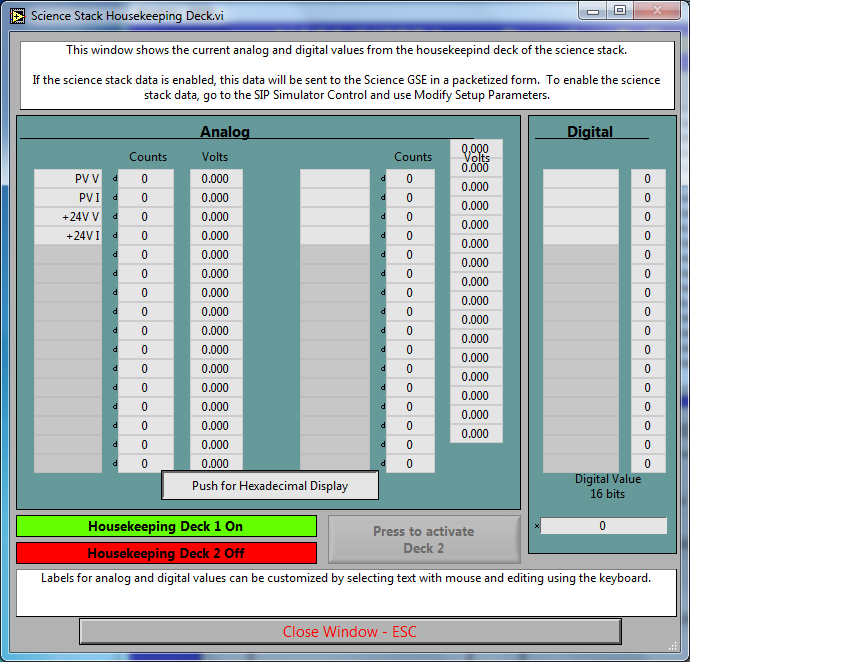
\includegraphics{housekeepingWindow.png}}
    \caption{The SIP Simulator science stack housekeeping window.}
    \label{fig:hkWindow}    
  \end{figure}

  To convert the readings to actual voltages the following conversion factors are used. Hmmm... these numbers need to be checked they don't look right to me.
  \begin{itemize}
  \item PV V  == Count * 0.065065
  \item PV I == Count * 0.081818
  \item +24V V == Count * 0.392150
  \item +24 V I == Count * 0.130440
  \end{itemize}

  The SIP Simulator can also provide a monitor of the rate of high rate data sent by the instrument. This is available from the {\verb TDRSS High Rate Monitor.vi} window shown in Figure~\ref{fig:highRateWindow}.
     
  \begin{figure}[hbt]
    \centering
    \resizebox{\textwidth}{!}{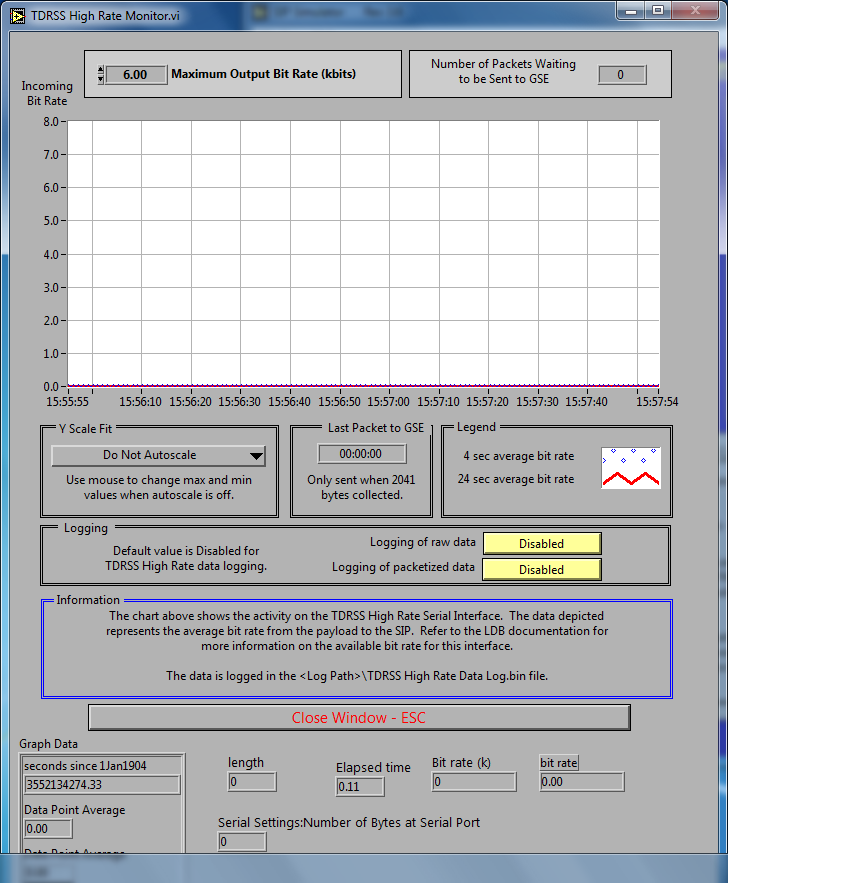
\includegraphics{highRateWindow.png}}
    \caption{The SIP Simulator TDRSS High Rate window.}
    \label{fig:highRateWindow}    
  \end{figure}
  

\clearpage
\appendix
\section{SIP Simulator Configuration Files}
\subsection{Serial Port Setup.txt}
\begin{verbatim}
Sci Data port      = 21
Sci Data baud rate = 115200
Sci cmd port       = 22
Sci cmd baud rate  = 2400
Comm 1 port        = 23
Comm 1 baud rate   = 1200
Comm 2 port        = 24
Comm 2 baud rate   = 1200
TDRSS Hi Rate In port = 25
TDRSS Hi Rate In baud rate = 115200
Sci Stack port = 26
Sci Stack baud rate = 4800
\end{verbatim}
\subsection{Sci Decks.ini}
\begin{verbatim}
[Sci CMD Deck Addresses]
Uses 2 Decks?=False
Deck 1 Address=F7
Deck 2 Address=F8
Timed Deck Address=83
[Sci HSK Deck Addresses]
Uses 2 Decks?=False
Deck 1 Address=F3
Deck 2 Address=F4
\end{verbatim}
\subsection{Sci HSK Deck 1 Labels.txt}
\begin{verbatim}
PV V, PV I, +24V V, +24V I
,,,
,,,
\end{verbatim}



\end{document}
